\documentclass{beamer}
\usepackage[utf8]{inputenc}

% For algorithms
\usepackage{algorithm}
\usepackage{algorithmic}

\renewcommand{\algorithmicinput}{\textbf{Input:}}
\renewcommand{\algorithmicoutput}{\textbf{Output:}}

\usetheme{Warsaw}
\title[Large-Scale Learning of Embeddings]{Large-Scale Learning of Embeddings with Reconstruction Sampling}
\author{Yann N. Dauphin, Xavier Glorot, Yoshua Bengio}
\institute{Université de Montréal}
\date{July 1, 2011}
\begin{document}
\AtBeginSubsection[]
{
  \begin{frame}<beamer>
    \frametitle{Outline}
    \tableofcontents[currentsection,currentsubsection]
  \end{frame}
}

\begin{frame}
\titlepage
\end{frame}

\begin{frame}{Background}
\begin{itemize}
\item Surge of interest for unsupervised learning algorithms.
\item (Hinton, 2006) shows that using the representation extracted by RBMs
leads to superior classification..
\item (Ranzato, 2006), (Bengio, 2006), et al. extend this results.
\end{itemize}
\end{frame}

\begin{frame}{Motivation}
\begin{itemize}
\item How to scale these algorithms to very sparse and very large input data?
\end{itemize}
\end{frame}

\begin{frame}{Problem}

\begin{center}
	\begin{figure}[htbp]
		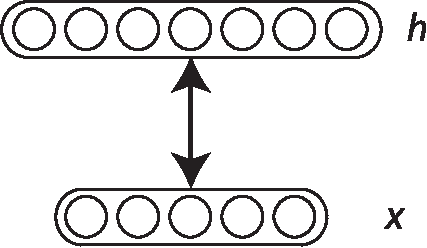
\includegraphics[width=4cm]{images/RBM.pdf}
	\end{figure}
\end{center}

\begin{itemize}
\item Typically, 2 expensive mappings need to be computed.
    \begin{itemize}
        \item Mapping from input to hidden representation.
        \item Mapping from hidden to input representation.
    \end{itemize}
\end{itemize}
\end{frame}

\frame{\frametitle{Outline} \tableofcontents}

\section{Related Work}
\begin{frame}{Related work}
\begin{itemize}
\item (Morin and Bengio, 2005) propose a Tree-structured predictors.
\item (Collobert and Weston, 2008) propose a ranking criterion estimated
by Monte-Carlo sample.
\end{itemize}
\end{frame}

\section{Denoising Auto-Encoders}
\begin{frame}{Denoising Auto-Encoders}
\begin{center}
	\begin{figure}[htbp]
		\resizebox{0.8\linewidth}{!}{\input{images/autoencoder_5.pstex_t}}
	\end{figure}
\end{center}

\begin{itemize}
\item Learning algorithm
for unsupervised feature extraction (Vincent, 2008).
\end{itemize}
\end{frame}

\begin{frame}{Denoising Auto-Encoders}
\begin{center}
	\begin{figure}[htbp]
		\resizebox{0.8\linewidth}{!}{\input{images/autoencoder_2.pdf_t}}
	\end{figure}
\end{center}

\begin{itemize}
\item ${\bf x} \in [0,1]^{d_x}$ is partially corrupted,
yielding $\tilde{\bf x} \sim q_{\mathcal{D}}(\tilde{\bf x}|{\bf x})$. 
\end{itemize}
\end{frame}

\begin{frame}{Denoising Auto-Encoders}
\begin{center}
	\begin{figure}[htbp]
		\resizebox{0.8\linewidth}{!}{\input{images/autoencoder_3.pdf_t}}
	\end{figure}
\end{center}

\begin{itemize}
\item Compute representation ${\bf h} = f_\theta(\tilde{\bf x})=\mathrm{sigmoid}(\underbrace{{\bf W}^{(1)}}_{d_h\times d_x} \tilde{\bf x} + \underbrace{{\bf b}^{(1)}}_{d_h \times 1})$
\end{itemize}
\end{frame}

\begin{frame}{Denoising Auto-Encoders}
\begin{center}
	\begin{figure}[htbp]
		\resizebox{0.8\linewidth}{!}{\input{images/autoencoder_4.pdf_t}}
	\end{figure}
\end{center}

\begin{itemize}
\item Compute reconstruction ${\bf z} = g_\theta({\bf h})=\mathrm{sigmoid}(\underbrace{{\bf W}^{(2)}}_{d_x\times d_h} {\bf h} + \underbrace{{\bf b}^{(2)}}_{d_x \times 1})$
\end{itemize}
\end{frame}

\begin{frame}{Denoising Auto-Encoders}
\begin{center}
	\begin{figure}[htbp]
		\resizebox{0.8\linewidth}{!}{\input{images/autoencoder_5.pstex_t}}
	\end{figure}
\end{center}

\begin{itemize}
\item Train to minimize the cross-entropy
$L({\bf x}, {\bf z}) = \sum_k^d H({\bf x}_k, {\bf z}_k)$.
\item (Vincent, 2011) shows this is equivalent to training an EBM.
\end{itemize}
\end{frame}

\begin{frame}{Denoising Auto-Encoders}
\begin{center}
	\begin{figure}[htbp]
		\resizebox{0.8\linewidth}{!}{\input{images/autoencoder_5.pstex_t}}
	\end{figure}
\end{center}

\begin{itemize}
\item Train to minimize the cross-entropy
$L({\bf x}, {\bf z}) = \sum_k^d H({\bf x}_k, {\bf z}_k)$.
\item (Vincent, 2011) shows this is equivalent to training an EBM.
\end{itemize}
\end{frame}

\section{Sparse Dot}
\begin{frame}{Sparse Dot}
\begin{itemize}
\item Reduce encoder complexity with sparse dot: $f_\theta \in O(d_s\times d_h)$
\end{itemize}
\end{frame}

\section{Reconstruction Sampling}
\begin{frame}{Reconstruction Sampling}
\begin{itemize}
\item Subsample the learning objective $L$.
\[
\hat{L}({\bf x}, {\bf z}) = \sum_k^d \frac{\hat{\bf p}_k}{{\bf q}_k} H({\bf x}_k, {\bf z}_k)
\]
\item $\hat{\bf p} \in \{0, 1\}^{d_x}$ with $\hat{\bf p} \sim
P(\hat{\bf p}|{\bf x})$ is the sampling pattern.
\item ${\bf q}$ is are scalar weights, and if ${\bf q}_k=E[\hat{\bf p}_k|k,{\bf x},\tilde{\bf x}]$ then
objective is unbiased since $E[\frac{\hat{\bf p}_k}{{\bf q}_k}|k,{\bf x},\tilde{\bf x}]=1$.
\item Reduces decoder complexity to $O(d_n\times d_h)$.
\end{itemize}
\end{frame}

\begin{frame}{Sampling Distribution}
\begin{itemize}
\item Minimize variance of the estimator.
\item Sample bits where  model will make an error.
\item Let ${\cal C}({\bf x},\tilde{\bf x})=\{k: {\bf x}_k=1 \;{\rm or}\;\tilde{\bf x}_k=1\}$, our
heuristic:
\begin{equation}
\label{eq:p}
P(\hat{\bf p}_k=1|{\bf x}_k) = \left\{ \begin{array}{ll} 1 & {\rm if}\; k \in {\cal C}({\bf x},\tilde{\bf x}) \nonumber\\
                                              |{\cal C}({\bf x},\tilde{\bf x})|/d_x & otherwise
              \end{array} \right.
\end{equation}
\item Sample all 1s and equal amount of 0s.
\end{itemize}
\end{frame}

\section{Implementation}
\begin{frame}{Implementation}
\begin{itemize}
\item The decoder is implemented as:
\[
{\bf z} = \mathrm{sigmoid}(\texttt{SamplingDot}({\bf h}, {\bf W}^{(2)}, \hat{\bf p}) + {\bf b}^{(2)})
\]
\vspace{-0.5cm}
\begin{center}
\begin{minipage}{0.9\textwidth}
    \begin{algorithm}[H]
    \caption{\texttt{SamplingDot}(${\bf A}$, ${\bf B}$, ${\bf C}$)}
    \begin{algorithmic}
    \INPUT ${\bf A} = [A_{ij}]_{M\times K}$, ${\bf B} = [B_{ij}]_{N\times K}$, ${\bf C} = [C_{ij}]_{M\times N}$
    \OUTPUT ${\bf D} = [D_{ij}]_{M\times N}$
    \STATE
    \FOR{$m = 1$ {\bf to} M}
        \FOR{$n = 1$ {\bf to} N}
            \IF {${\bf C}_{mn} \neq 0$}
                \STATE ${\bf D}_{m} \gets \texttt{DOT}({\bf A}_{m}, {\bf B}_{n})$
            \ENDIF
        \ENDFOR
    \ENDFOR
    \end{algorithmic}
    \end{algorithm}
\end{minipage}
\end{center}
\end{itemize}
\end{frame}

\section{Experimental Results}
\begin{frame}{Datasets}
\begin{itemize}
\item {\bf Amazon Multi-Domain Sentiment Dataset.} More than $340,000$ product reviews 
on $25$ different domains.
\item {\bf Reuters Corpus Volume I} (RCV1-v2). Over 800,000 real-world
news wire stories represented in bag-of-words vectors with 47,236 dimensions.
\end{itemize}
\end{frame}

\begin{frame}{Convergence}
\begin{center}
\begin{minipage}{.7\textwidth}
\begin{center}
  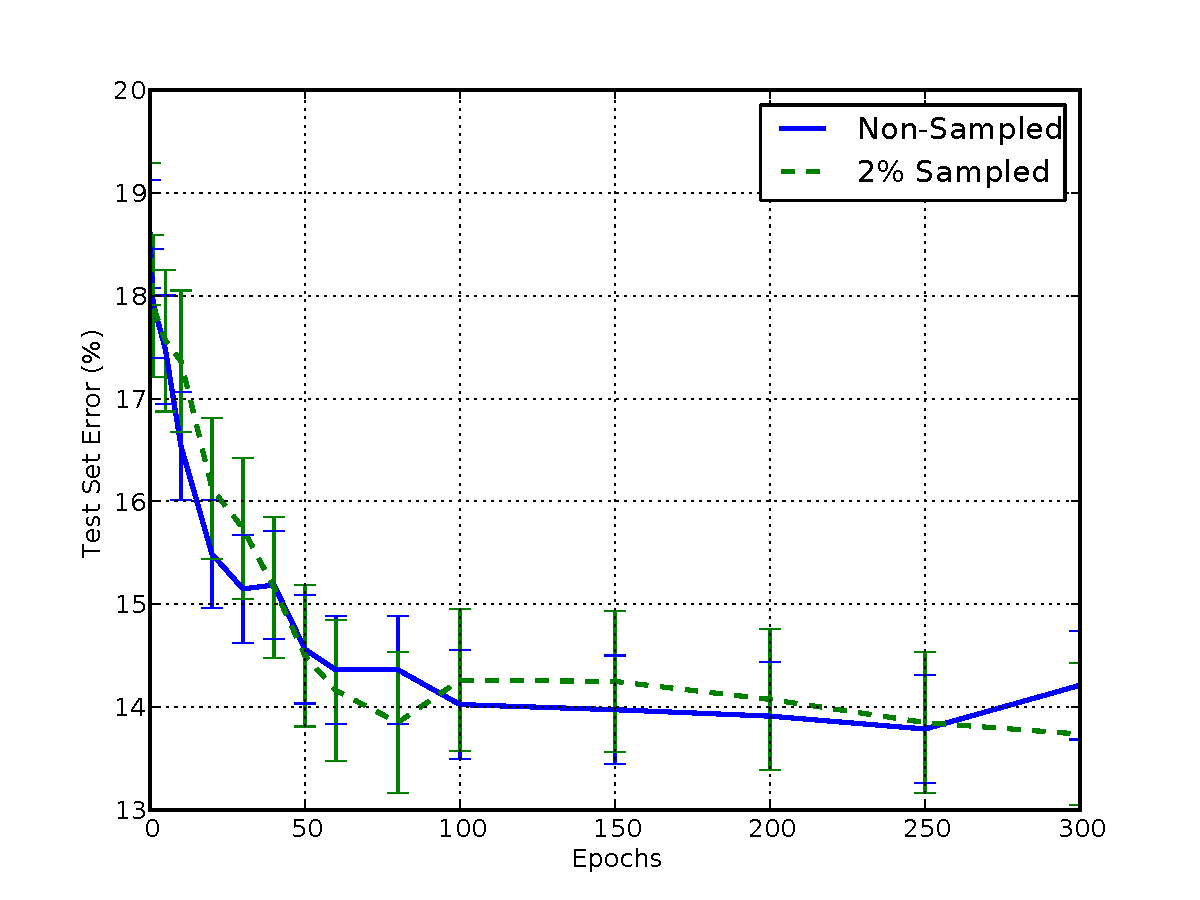
\includegraphics[width=.95\textwidth]{images/amazon_convergence.pdf}\\
  {\bf Amazon}
\end{center}
\end{minipage}
\end{center}
\end{frame}

\begin{frame}{Bias}
\begin{center}
\begin{minipage}{.7\textwidth}
\begin{center}
  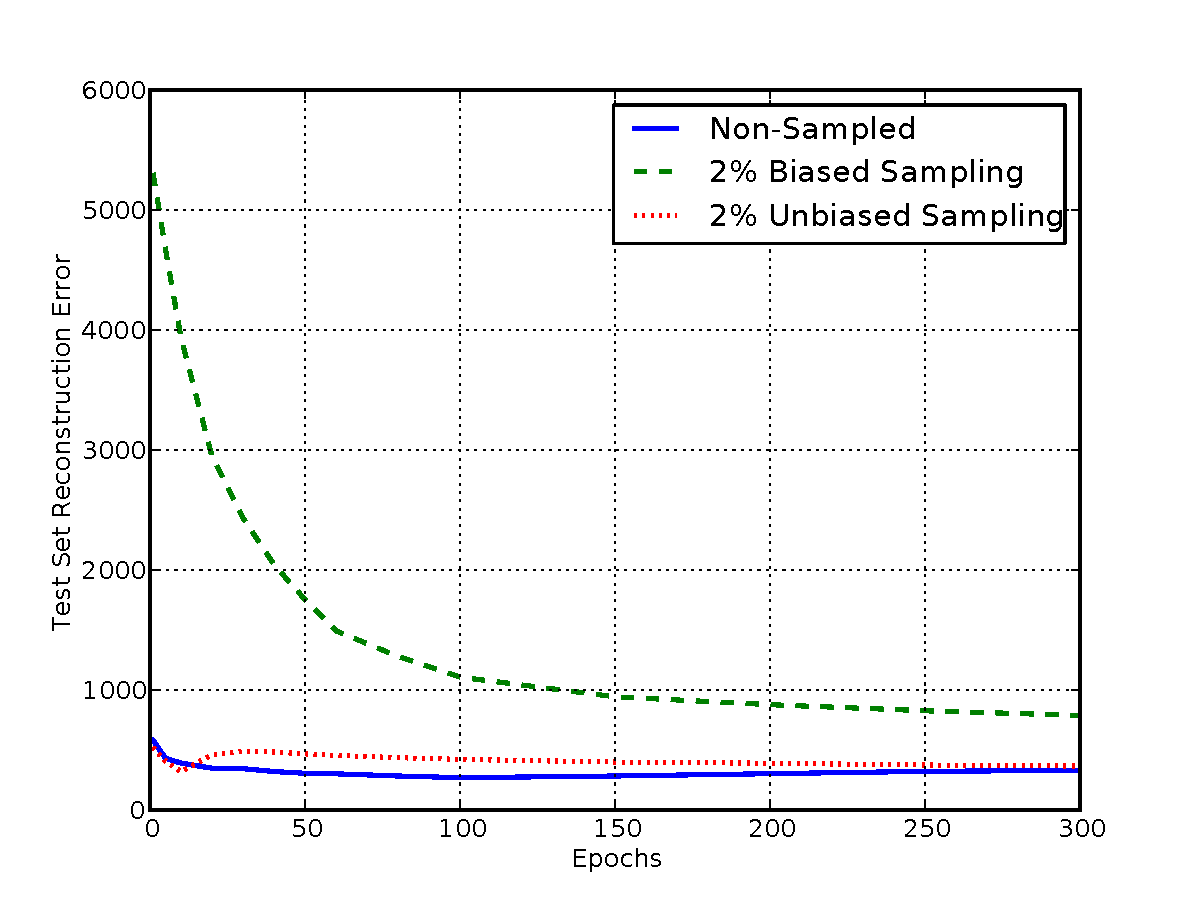
\includegraphics[width=.95\textwidth]{images/amazon_bias.pdf}\\
  {\bf Amazon}
\end{center}
\end{minipage}
\end{center}
\end{frame}

\begin{frame}{Quality of the representation}
\begin{center}
\begin{minipage}{.7\textwidth}
\begin{center}
  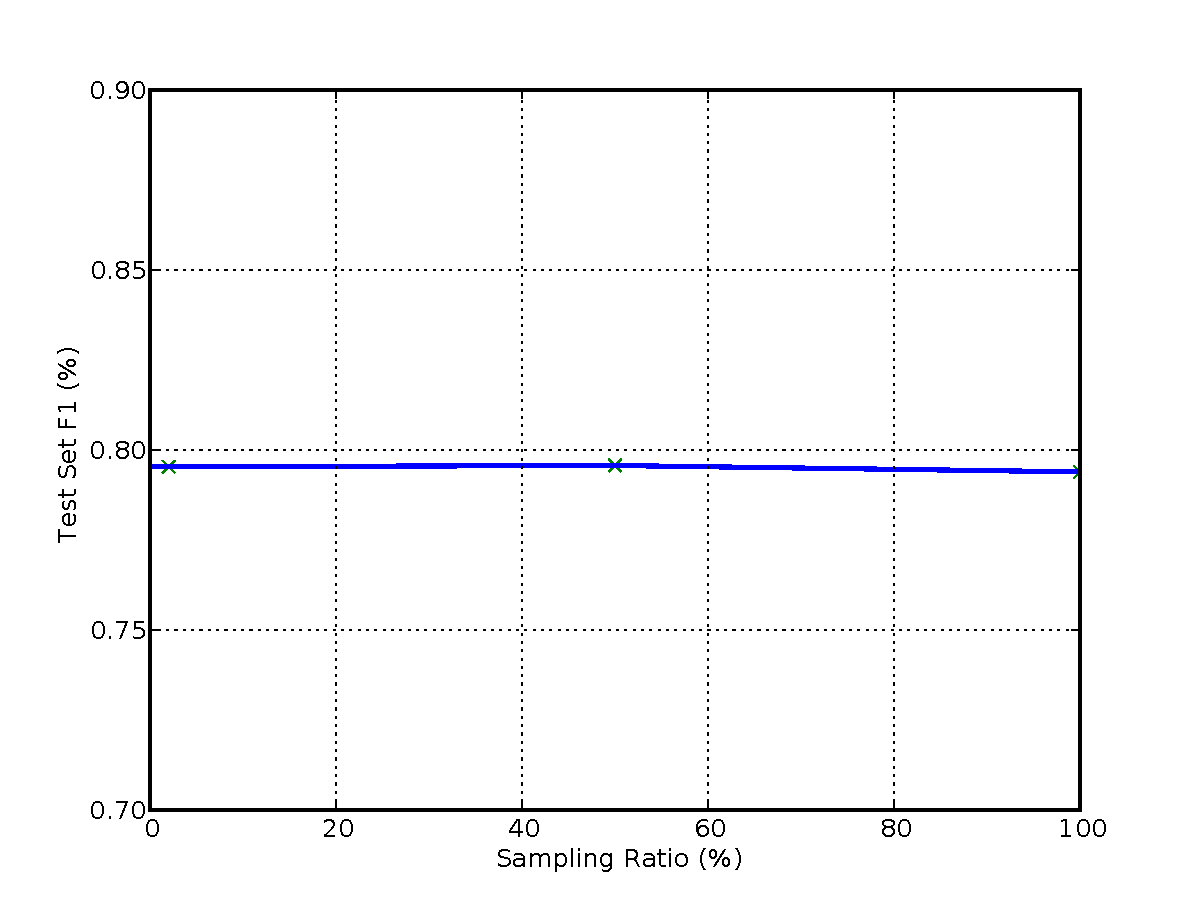
\includegraphics[width=.95\textwidth]{images/rcv1_generalization.pdf}\\
  {\bf RCV1-v2}
\end{center}
\end{minipage}
\end{center}
\end{frame}

\begin{frame}{Speed-ups}
\begin{center}
\begin{minipage}{.7\textwidth}
\begin{center}
  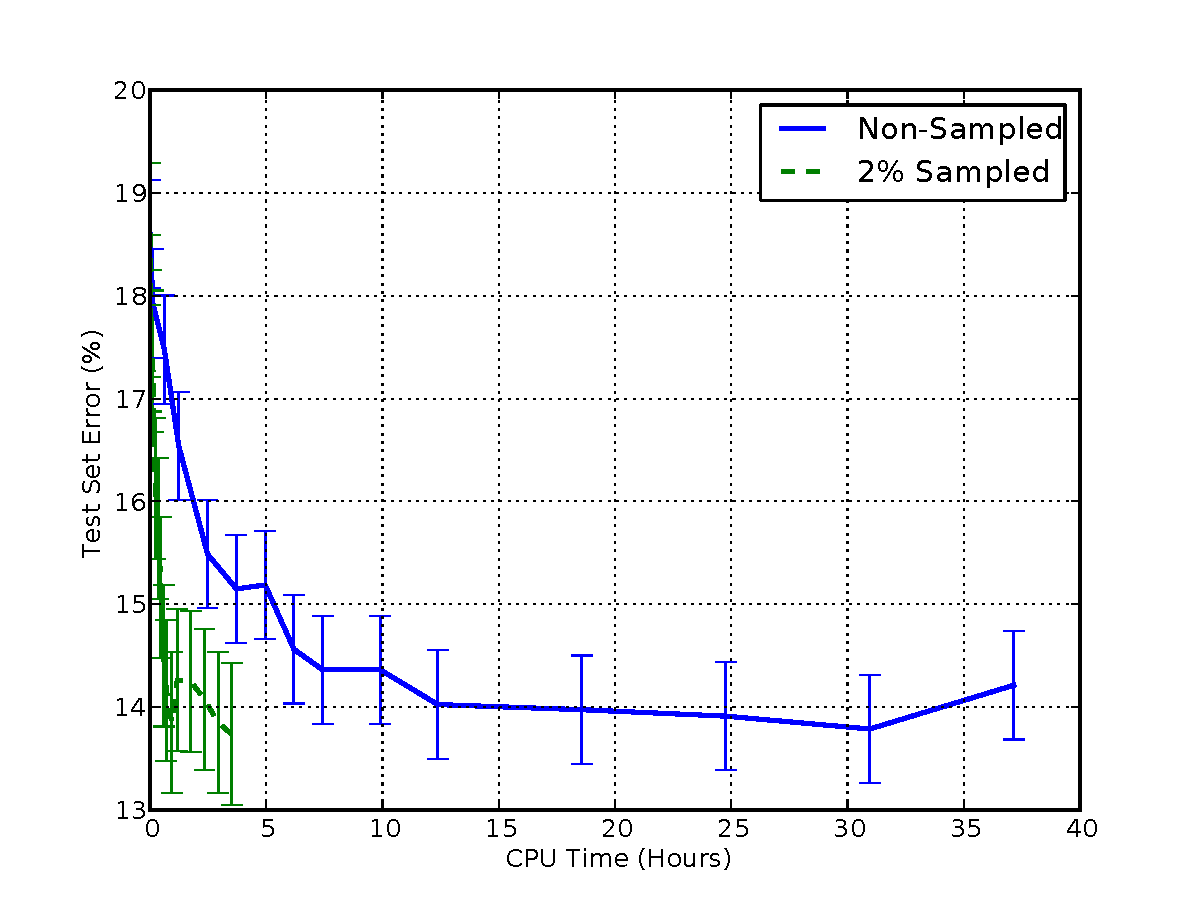
\includegraphics[width=.95\textwidth]{images/amazon_speedup.pdf}\\
  {\bf Amazon}
\end{center}
\end{minipage}
\end{center}
\end{frame}

\begin{frame}{Speed-ups}
\begin{center}
\begin{minipage}{.7\textwidth}
\begin{center}
  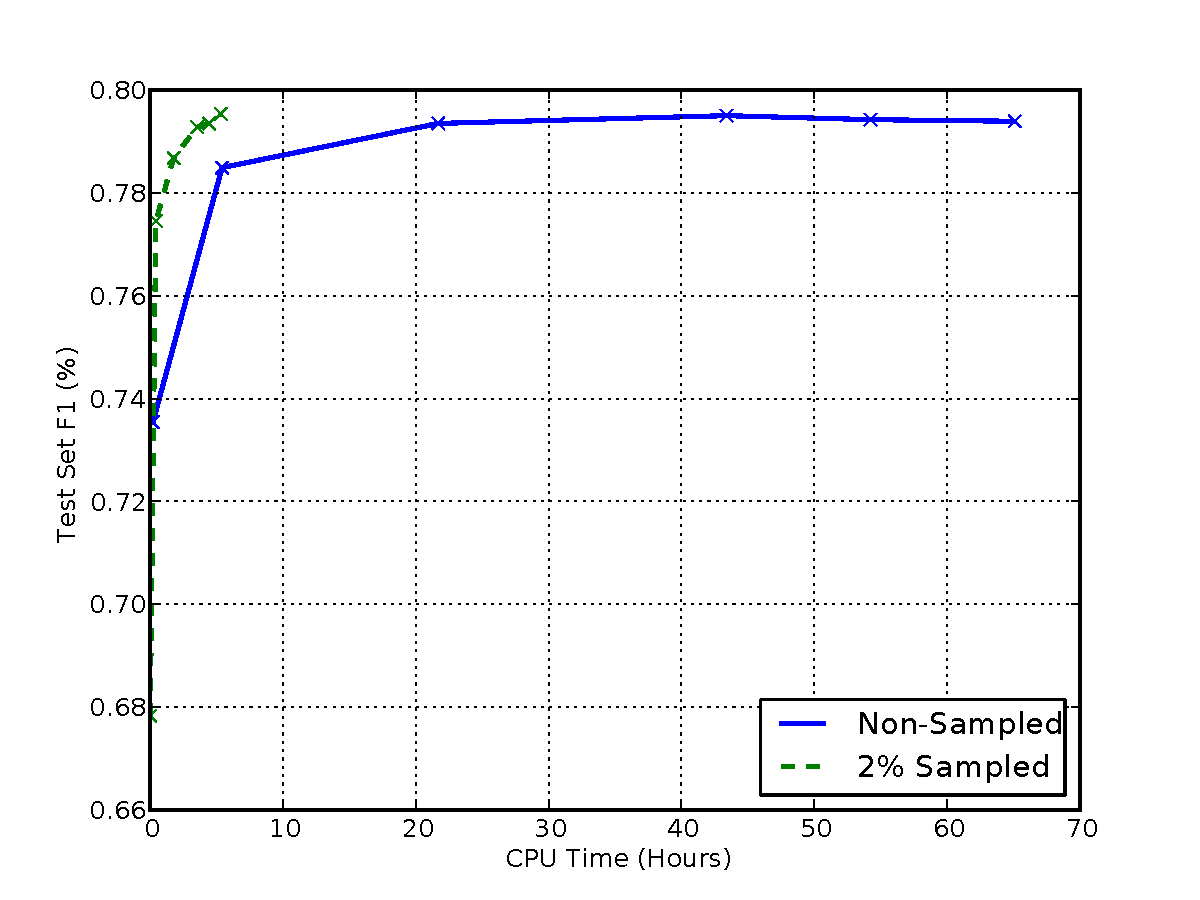
\includegraphics[width=.95\textwidth]{images/rcv1_speedup.pdf}\\
  {\bf RCV1-v2}
\end{center}
\end{minipage}
\end{center}
\end{frame}

\begin{frame}{Speed-ups}
\begin{center}
\begin{minipage}{.7\textwidth}
\begin{center}
  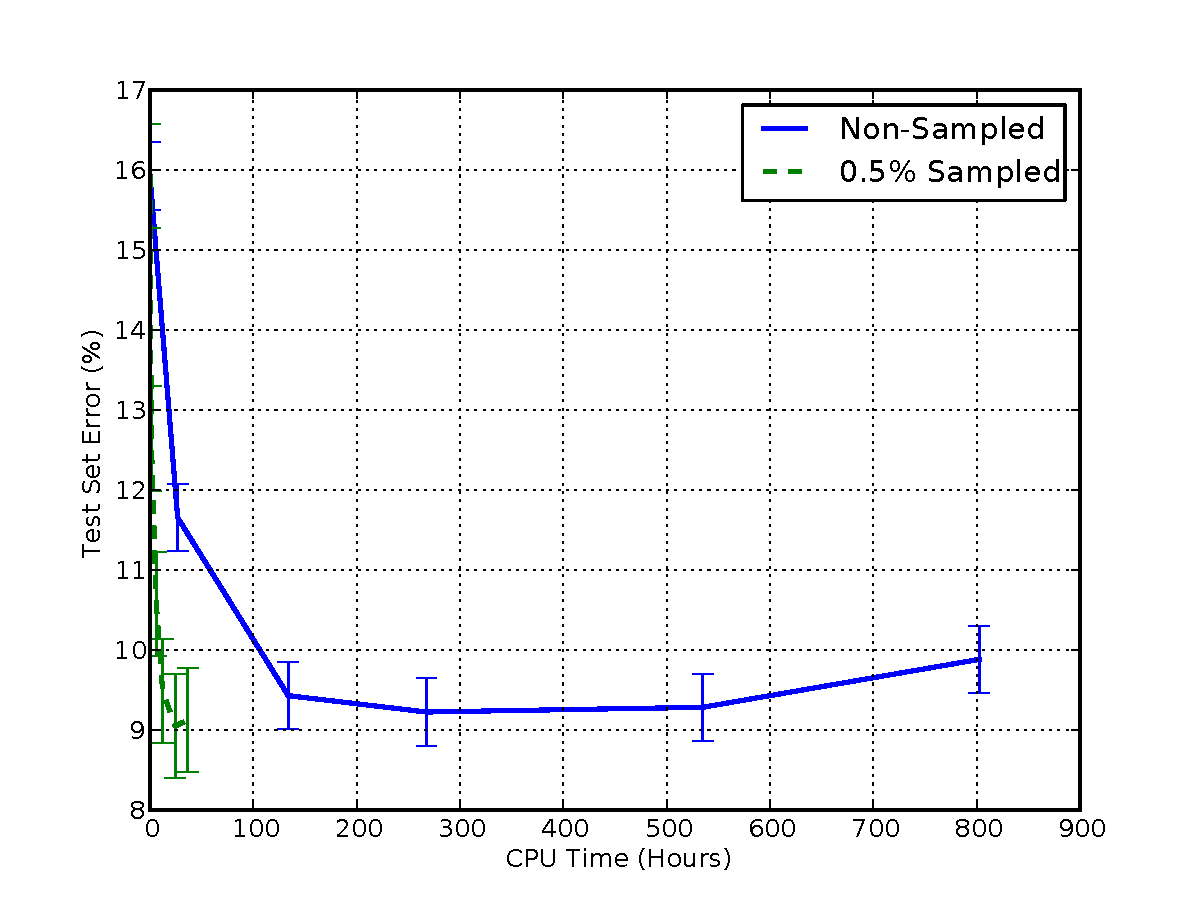
\includegraphics[width=.95\textwidth]{images/fullamazon_speedup.pdf}\\
  {\bf Full Amazon}
\end{center}
\end{minipage}
\end{center}
\end{frame}

\section{Conclusion}
\begin{frame}{Conclusion}
\begin{itemize}
\item Introduced simple speed-up technique.
\item Unbiased estimator.
\item Same quality of representation.
\item Speed-ups up to 20x.
\end{itemize}
\end{frame}

\end{document}
